%---------------------------------------------------------------------------------------------------
%		main.tex
%
%	This is the main file of the chapter that talk about the measurments.
%
%	Author: Andrea Meneghinello
% Version: 0.1
%	Table of changes:
%		21/03/2016 -> document definition
%---------------------------------------------------------------------------------------------------
\chapter{Measurements}
\label{cap:measurements}
In order to offer high level of service a \ac{paas} provider must install, on its physical systems,
a virtualization layer that is able to exploit the underlying hardware as better as it can. Is not
sufficient that the layer virtualize the fundamental assets (see Section
\ref{sec:background-virtualization-assets}), it must contain also a good resource scheduler. It should
be able to schedule the different workloads in devices that have hardware resources conform with the
current workload in order to assure elasticity.

In this chapter we want to try to isolate and understand the overhead introduced by \ac{vm}s
(specifically \ac{kvm}) and containers (specifically Docker). The fact that Linux is able to host
both \ac{vm}s and Docker containers creates the opportunity for an apple-to-apple comparison between
these two virtualization technologies.

Thus, in the following sections we report the results collected during the comparison tests. Each 
section illustrate the purpose of the test, illustrate the collected results and try to explain them.

%---------------------------------------------------------------------------------------------------
%		introduction.tex
%
%	This is the main file of the chapter that talk about elasticity.
%
%	Author: Andrea Meneghinello
% Version: 0.1
%	Table of changes:
%		17/03/2016 -> document definition
%---------------------------------------------------------------------------------------------------
\section{Introduction}
\label{sec:elasticity-introduction}
A requirement for distributed services is availability: they must remain regularly available to be
used by as many customers as needed with \keyword{acceptable performance} and \keyword{scalability}.
Distributed services and systems have always been required to be scalable. Replication of services
components, in order to balance the workload arriving to each replica, has been the chosen approach.

Services needed to be carefully designed in order to minimize synchronization needs among their
components with the aim of not blocking their execution. Evidently, unlimited scalability could not be
achieved since it requires infinite infrastructure resources. So, traditionally, scalability of a
service depends on its software architecture being limited by the amount of hardware resources secured
in the data-centre where it was deployed.

As we have seen in the previous chapter, the advent of cloud computing partially broke those limits, but
elasticity management remains not trivial.

According to the \ac{nist} definition (given in Section
\ref{sec:background-cloudComputing-cloudServiceModels}), \ac{paas} gives freedom to the customer regarding
application reconfiguration, since end-users should only deal with the general ``configuration settings
for the application-hosting environment'' but do not need to worry about the mechanism being needed
for implementing those reconfigurations. Reconfiguration management is the responsibility of \ac{paas}
providers. Since every cloud service should be elastic (accordingly with cloud definition), this mean
that \ac{paas} providers should deal with many mechanism that automate the service scalability and
adaptability.

However, the level of automation needed to approach a cost-optimal exploitation of the service is still
changing nowadays because of the many aspects that should be considered. On one hand, scalability
decisions must match what has been stated in the \ac{sla}. This means that those decisions should be
taken as soon as the workload or the service performance starts to vary, which strongly suggests the
need to include some workload prediction mechanism. Nevertheless, forecasting techniques are not perfect
hence, they should be complemented with other reactive mechanism; e.g. when the resulting service
performance level do not comply with what is being specified in the \ac{sla} or lead unnecessary
over-provisioning costs, service providers should take appropriate actions. Those actions may consist
in adding service instances or migrating those instances to better \ac{vm}s when service capacity
should be increased, or in the opposite case, in releasing instances when service capacity need to be
decreased.

One of the regular dimensions in \ac{sla}s is availability. Successful distributed services are
concurrently used by many customers. Service providers should guarantee service continuity, otherwise
service clients will not rely on that provider and they will look for another, more reliable, one.
Unfortunately, since complex software systems are always in need of modification, both platform and
service components need to be eventually updated in order to fix bugs, remove security vulnerabilities
or enhance their functionality. This software upgrading process might put at risk the availability levels
specified in a \ac{sla}. So, this is another source of trouble for service providers.



%---------------------------------------------------------------------------------------------------
%		cpu.tex
%
%	This is file contains the cpu measurements.
%
%	Author: Andrea Meneghinello
% Version: 0.1
%	Table of changes:
%		21/03/2016 -> document definition
%---------------------------------------------------------------------------------------------------
\section{\acs{cpu} benchmark}
\label{sec:measurements-cpu}
By means of Linpack benchmark tool we want to measure the \acs{cpu} performance of both virtualization
environments. In order to have a basis for comparison we initially have executed the tool on the native
machine and then in various interesting environments, including:

\begin{enumerate}
	\item{one Docker container over the native \acs{os};}
	\item{one \ac{kvm} \ac{vm} with Hyper-Threading enabled;}
	\item{one \ac{kvm} \ac{vm} with Hyper-Threading disabled;}
	\item{one Docker container inside a \ac{kvm} \ac{vm} with Hyper-Threading enabled;}
	\item{one Docker container inside a \ac{kvm} \ac{vm} with Hyper-Threading disabled.}
\end{enumerate}

Even if running a container inside a \ac{vm} creates a double layer of virtualization, we also evaluated
these scenarios (2,3,4,5) because this is the only available solution if we choose a \ac{iaas} (like 
\ac{aws}) instead a \ac{paas} provider.

The \acs{cpu} tests were performed twice. The first time they where executed in complete isolation
in order to measure the overhead introduced by the virtualization layer; instead the second time they
were performed inserting an annoyance element that, casually, raised up and disturbed our computations.
This last one was performed to measure how the two virtualization types are able to adapt themselves
when they need to share the underlying hardware resources.

\subsection{Hyper-Threading Technology}
\label{sec:measurements-cpu-hyperThreadingTechnology}
Hyper-Threading (officially called Hyper-Threading Technology) is Intel's proprietary simultaneous
multi-threading implementation used to improve parallelization of computations performed on x86
microprocessors. Figure \ref{img:measurements-cpu-hyperThreading} shows an example of execution with
Hyper-Threading enabled.

\begin{figure}
	\centering{}
	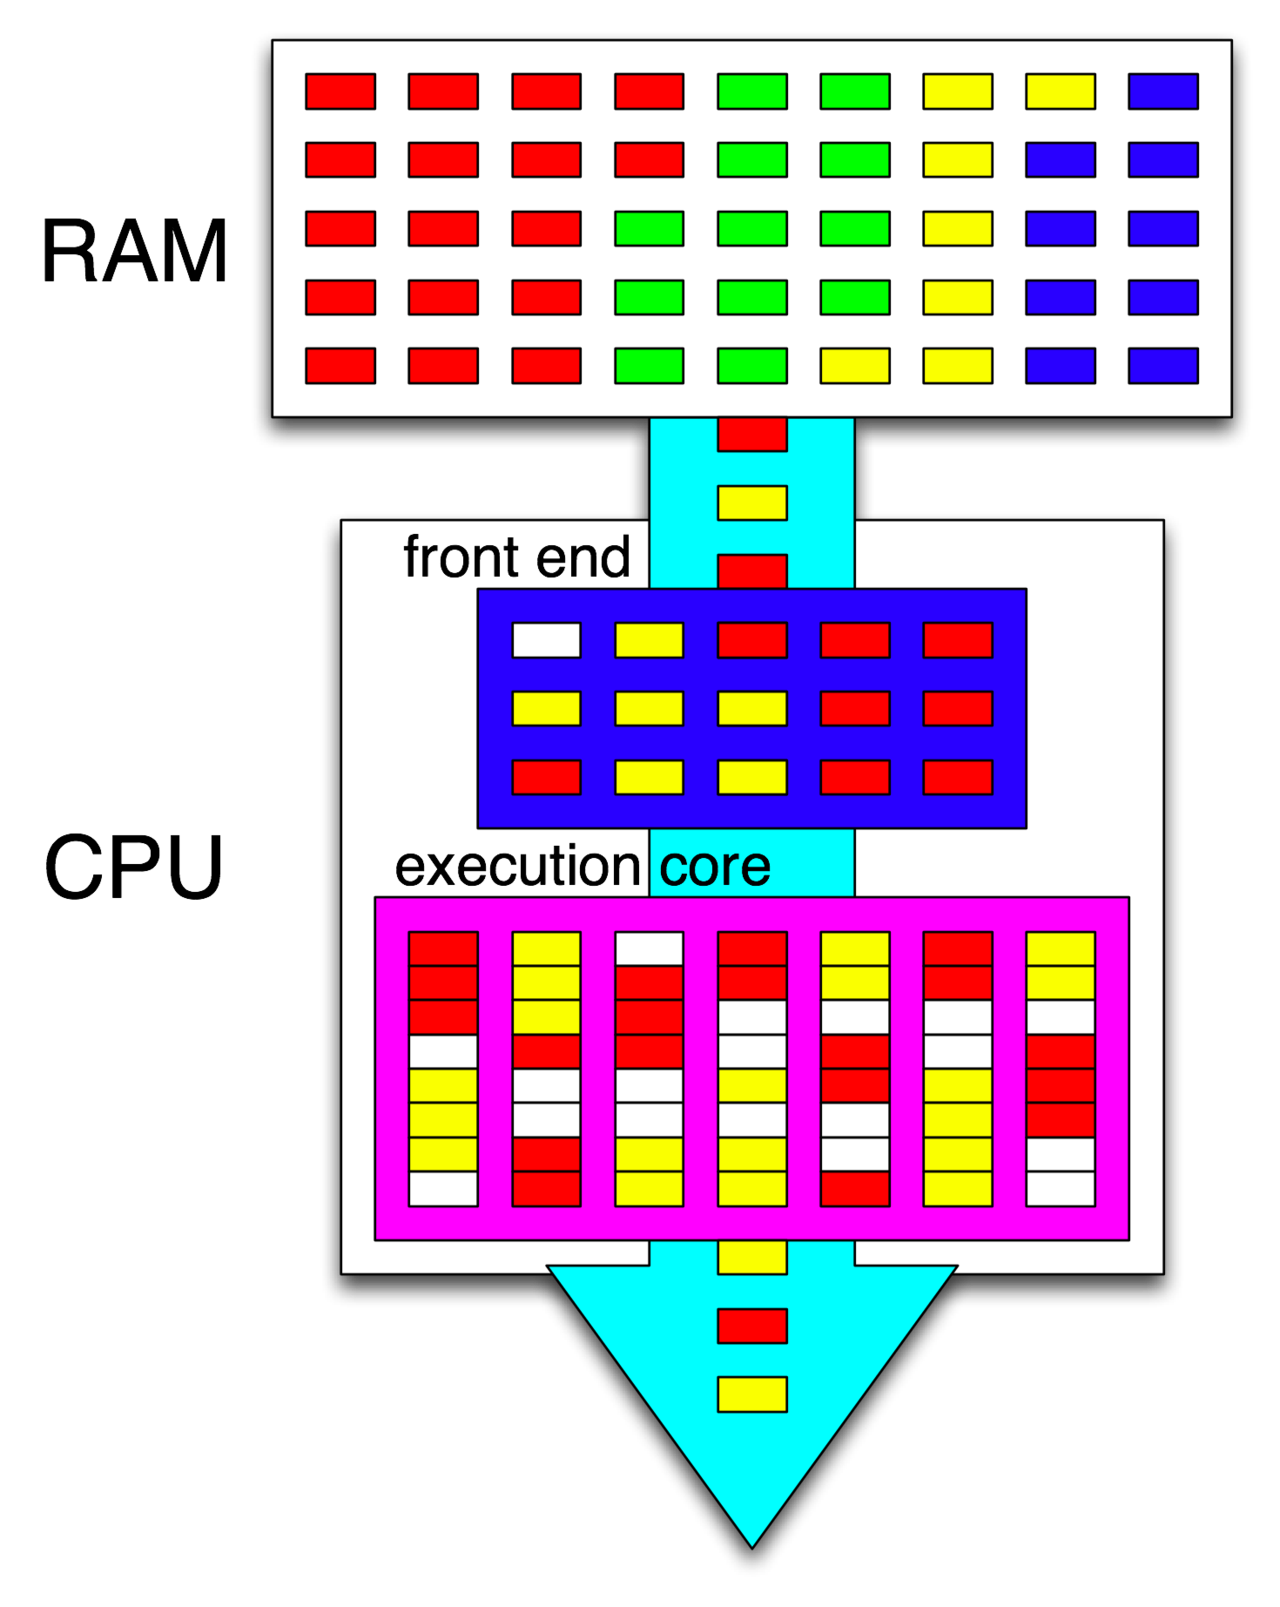
\includegraphics[width=0.35\textwidth]{chapters/measurements/images/hyper-threading.png}
	\caption[Overview of Intel Hyper-Threading]{A high-level depiction of the Intel's Hyper-Threading
		Technology: instructions are fetched from RAM (differently coloured boxes represent the instructions
		of four different programs), decoded and reordered by the front end (white boxes represent pipeline bubbles),
		and passed to the execution core capable of executing instructions from two different programs during
		the same clock cycle \cite{hyperthreading}.}
	\label{img:measurements-cpu-hyperThreading}
\end{figure}

For each processor core that is physically present, the \acs{os} addresses two virtual or logical cores,
and shares the workload between them when possible. The main function of Hyper-Threading is to increase
the number of independent instructions in the pipeline; it takes advantage of super-scalar architecture,
in which multiple instructions operate on separate data in parallel. With Hyper-Threading, one physical
core appears as two processors to the \acs{os}, allowing concurrent scheduling of two processes
per core. In addition, two or more processes can use the same resources: if resources for one process
are not available, then another process can continue if its resources are available.

In addition to requiring simultaneous multi-threading support in the \acs{os}, Hyper-Threading can be
properly utilized only with any \acs{os} specifically optimized for it. Furthermore, Intel recommends
to disable it when we are using an \acs{os} unaware of this hardware feature or in virtualized
environments.

\subsection{Linpack benchmark}
\label{sec:measurements-cpu-linpack}
\ac{hpl} \cite{linpackBenchmark} is a benchmark that measures the performance of a node or a cluster
using a workload that is characteristic of some scientific and technical applications. It is able to
solve a dense system of linear equations. Each system is represented as a matrix that will be divided
into smaller pieces, called ``tiles'', and distributed across the available processors or cluster's
nodes. Final performance is reported as the number of \ac{flops} achieved by the system. Users are able
to configure the benchmark varying the size of the problem and a number of parameters that describe
how the problem is solved. Some of the parameters describe how the problem is decomposed into tiles,
and how those tiles are distributed over the available resources.

The tool itself is a collection of subroutines that analyse and solve linear equations and linear
least-square problems. Originally was designed for supercomputers in the 1970s and early 1980s, it is able
to solves linear systems whose matrices are general, banded, symmetric indefinite, symmetric positive
definite, triangular, and triangular square. Linpack tool is built upon \ac{blas} package. It
uses LU factorization algorithm, similar to a technique commonly taught in college Linear Algebra courses,
called Gaussian elimination, but it is significantly improved to increase its numerical stability and
its performance.

Linpack library has largely been replaces by Lapack, which extends and improves upon the routines. In
Lapack, the routines have been carefully rewritten and tuned to take advantage of processors' cache,
available cores and relatively few references actually go to memory. In our tests, we used the
double-precision \ac{hpl} benchmark provided by Intel.

The benchmark produce a set of interesting values that describe the \ac{sut}, they are:

\begin{itemize}
	\item{\keyword{$R_{max}$}: which is the maximum measured performance in \ac{gflops};}
	\item{\keyword{$N$}: which represents the number of equations used to obtain $R_{max}$;}
	\item{\keyword{$R_{peak}$}: which represents the theoretical peak performance for the system; usually
		it is obtained by multiplying the number of processor cores, the processor frequency and the
		theoretical number of 64-bit vector floating-point results per clock;}
	\item{\keyword{$N_{1/2}$}: which represents the number of equations required to obtains one-half
		of the $R_{max}$ performance; it indicate the robustness of the system; a system with
		a small $N_{1/2}$ is able to operate well over a wide range of problems.}
\end{itemize}

With the preceding values we are also able to find the efficiency of the system through:

\begin{center}
	\begin{equation}
		efficienty = \frac{R_{max}}{R_{peak}}
	\end{equation}
\end{center}

Linpack \ac{hpl} is primarily a processor-core-intensive benchmark. It heavily exercises the vector
floating-point unit of each processor core. The faster the processor core and the more cores that are
available, the better are the benchmark performance. Data is moved from a memory into cache and used
heavily form cache, so larger caches do help. With current cache sizes of 1MB or more, most of
the current working data set already fits into cache, so memory performance is not seen as a major
factor in determining final performance. Instead a factor that affect the final performance is how
the tiles are defined and distributed.

The tool is used every year to compute the list of the major 500 super-computers in the world. After many
execution developers assert that good values are obtained finding a value for $N$ which saturate the
$80\%$ of the available main memory.

\subsection{Configuration}
\label{sec:measurements-cpu-configuration}
In order to respect the general convention (see in Section \ref{sec:measurements-cpu-linpack}) we found
a value for $N$ that is able to generate a system of linear-equations that saturate approximately the
$80\%$ of the available main memory; that is:

\begin{center}
	\begin{equation}
		N = \sqrt{\frac{available RAM * 1024^3}{8}}
	\end{equation}
\end{center}

that in our case correspond to $82\,897$ equations per system.

\subsection{Results}
\label{sec:measurements-cpu-results}
After executing the test in the environments described in Section \ref{sec:measurements-cpu} with the
configuration described in Section \ref{sec:measurements-cpu-configuration} we collected the execution
times (illustrated in Table \ref{tbl:measurements-cpu-results-time}) and the \acs{cpu}
capacity (illustrated in Table \ref{tbl:measurements-cpu-results-capacity}) for each listed
environment.

Actually the ``test number'' value, reported in the first column of each table, refers to test cases
of that list.

\begin{center}
	\begin{tabular}{| l | r | r | r | r | r |}
		\hline
		\multirow{2}{*}{Test num} &   \multicolumn{5}{c|}{\keyword{\acs{cpu} capacity without contention (\acs{gflops})}}   \\ \cline{2-6}
		                          & \textit{Min} & \textit{Max} & \textit{Avg} & \textit{Std. Dev.} & \textit{\% upon tot.} \\ \hline
		\textit{native}           & $286.3051$   & $303.0076$   & $293.1930$   & $6.3289$           & $100.000$             \\ \hline
		\textit{2}                & $266.4806$   & $306.6239$   & $285.4630$   & $12.8306$          & $97.364$              \\ \hline
		\textit{3}                & $84.3842$    & $86.4793$    & $85.9023$    & $0.7661$           & $29.299$              \\ \hline
		\textit{4}                & $94.1811$    & $95.3780$    & $95.0015$    & $0.4321$           & $32.402$              \\ \hline
		\textit{5}                & $84.2199$    & $88.0320$    & $85.9904$    & $1.3263$           & $29.329$              \\ \hline
		\textit{6}                & $91.5771$    & $94.2375$    & $93.1346$    & $0.8818$           & $31.766$              \\ \hline\hline
		\multirow{2}{*}{Test num} &    \multicolumn{5}{c|}{\keyword{\acs{cpu} capacity with contention (\acs{gflops})}}     \\ \cline{2-6}
		                          & \textit{Min} & \textit{Max} & \textit{Avg} & \textit{Std. Dev.} & \textit{\% upon tot.} \\ \hline
		\textit{native}           & $226.1955$   & $310.3253$   & $262.9988$   & $27.3098$          & $100.000$             \\ \hline
		\textit{2}                & $239.2409$   & $294.9315$   & $262.7408$   & $18.8278$          & $99.902$              \\ \hline
		\textit{3}                & $72.9531$    & $85.5957$    & $79.1688$    & $4.4305$           & $30.102$              \\ \hline
		\textit{4}                & $71.0966$    & $86.6270$    & $82.5354$    & $5.8239$           & $31.382$              \\ \hline
		\textit{5}                & $76.7307$    & $79.6143$    & $78.2996$    & $1.0309$           & $29.772$              \\ \hline
		\textit{6}                & $84.4720$    & $91.2945$    & $88.8362$    & $2.2995$           & $33.778$              \\ \hline
	\end{tabular}
	\captionof{table}{Resume of the \acs{cpu} capacity benchmark.}
	\label{tbl:measurements-cpu-results-capacity}
\end{center}

\begin{figure}
	\centering{}
	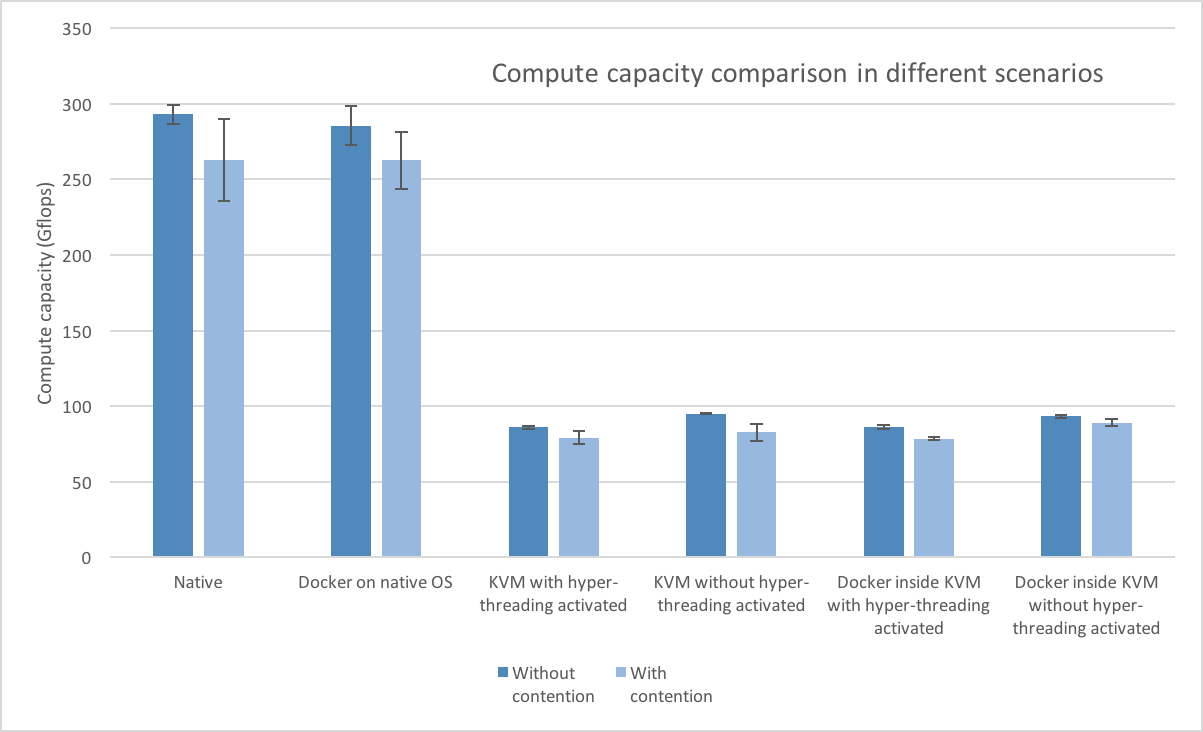
\includegraphics[width=0.75\textwidth]{chapters/measurements/images/cpu-capacity.png}
	\caption[Compute - resume of capacity benchmark]{Resume of \acs{cpu} capacity benchmark.}
	\label{img:measurements-cpu-results-capacity}
\end{figure}

In regard of \acs{cpu} capacity we can observe both from Table \ref{tbl:measurements-cpu-results-capacity}
and from chart \ref{img:measurements-cpu-results-capacity} that the \acs{os}-level virtualization,
provided by Docker, is able to exploit very well the \acs{cpu} capacity, both without and with contention.
The losses provided by that virtualization layer are approximatively from 1 to 3\%. Quite another thing is
the  hardware-level virtualization on which we collected losses approximatively from 68 to 71\% of the
\acs{cpu} compute capacity. This happens because the Linpack benchmark is highly adaptive and uses
system-provided information to tune itself to the architecture upon which it is running. The hardware-level
virtualization hides the totality of hardware information so the benchmark have to use generic algorithms
instead using optimizations.

In the matter of the double virtualization layer provided by inserting a Docker container inside a
\ac{kvm} \ac{vm} we do not find big differences from the execution without Docker inside the \ac{vm}.
In fact, we expect to find this results inasmuch Docker containers executing at the same level
of the \acs{os} on which they are based.

With respect to the capability of adapt themselves we have found better performance using
hardware-level virtualization instead the \acs{os}-level one, as the small standard deviation values
shows. We can affirm that this happens because the hardware-level virtualization is able to ``pin''
the underlying hardware resources to avoid over-scheduling.

Finally, as we expected executing relevant computation in virtualized environment that uses the Intel
Hyper-Threading Technology produces additional losses in \acs{cpu} capacity. Thus, the choice of
cloud provider of disable this feature produce a light increase of the performance.

\begin{center}
	\captionof{table}{Resume of \acs{cpu} capacity execution time.}
	\begin{tabular}{| l | r | r | r | r | r |}
		\hline
		\multirow{2}{*}{Test num} &               \multicolumn{5}{c|}{\keyword{Time without contention (s)}}                \\ \cline{2-6}
		                          & \textit{Min} & \textit{Max} & \textit{Avg} & \textit{Std. Dev.} & \textit{\% upon tot.} \\ \hline
		\textit{native}           & $1\,253.393$ & $1\,326.514$ & $1\,295.949$ & $27.747$           & $100.000$             \\ \hline
		\textit{2}                & $1\,238.611$ & $1\,425.198$ & $1\,333.098$ & $59.504$           & $102.867$             \\ \hline
		\textit{3}                & $4\,391.658$ & $4\,500.697$ & $4\,421.514$ & $39.941$           & $341.180$             \\ \hline
		\textit{4}                & $3\,981.921$ & $4\,032.526$ & $3\,997.138$ & $18.337$           & $308.433$             \\ \hline
		\textit{5}                & $4\,314.201$ & $4\,509.476$ & $4\,417.676$ & $67.989$           & $340.883$             \\ \hline
		\textit{6}                & $4\,039.111$ & $4\,147.189$ & $4\,080.002$ & $36.749$           & $314.827$             \\ \hline\hline
		\multirow{2}{*}{Test num} &                 \multicolumn{5}{c|}{\keyword{Time with contention (s)}}                 \\ \cline{2-6}
		                          & \textit{Min} & \textit{Max} & \textit{Avg} & \textit{Std. Dev.} & \textit{\% upon tot.} \\ \hline
		\textit{native}           & $1\,223.837$ & $1\,679.024$ & $1\,459.127$ & $146.186$          & $100.000$             \\ \hline
		\textit{2}                & $1\,287.715$ & $1\,587.470$ & $1\,452.694$ & $100.854$          & $99.559$              \\ \hline
		\textit{3}                & $4\,436.996$ & $5\,205.913$ & $4\,770.323$ & $259.307$          & $326.930$             \\ \hline
		\textit{4}                & $4\,384.173$ & $5\,341.855$ & $4\,773.795$ & $356.586$          & $327.168$             \\ \hline
		\textit{5}                & $4\,770.345$ & $4\,956.926$ & $4\,870.700$ & $75.448$           & $333.809$             \\ \hline
		\textit{6}                & $4\,254.526$ & $4\,698.309$ & $4\,396.572$ & $161.418$          & $301.315$             \\ \hline
	\end{tabular}
	\label{tbl:measurements-cpu-results-time}
\end{center}

\begin{figure}
	\centering{}
	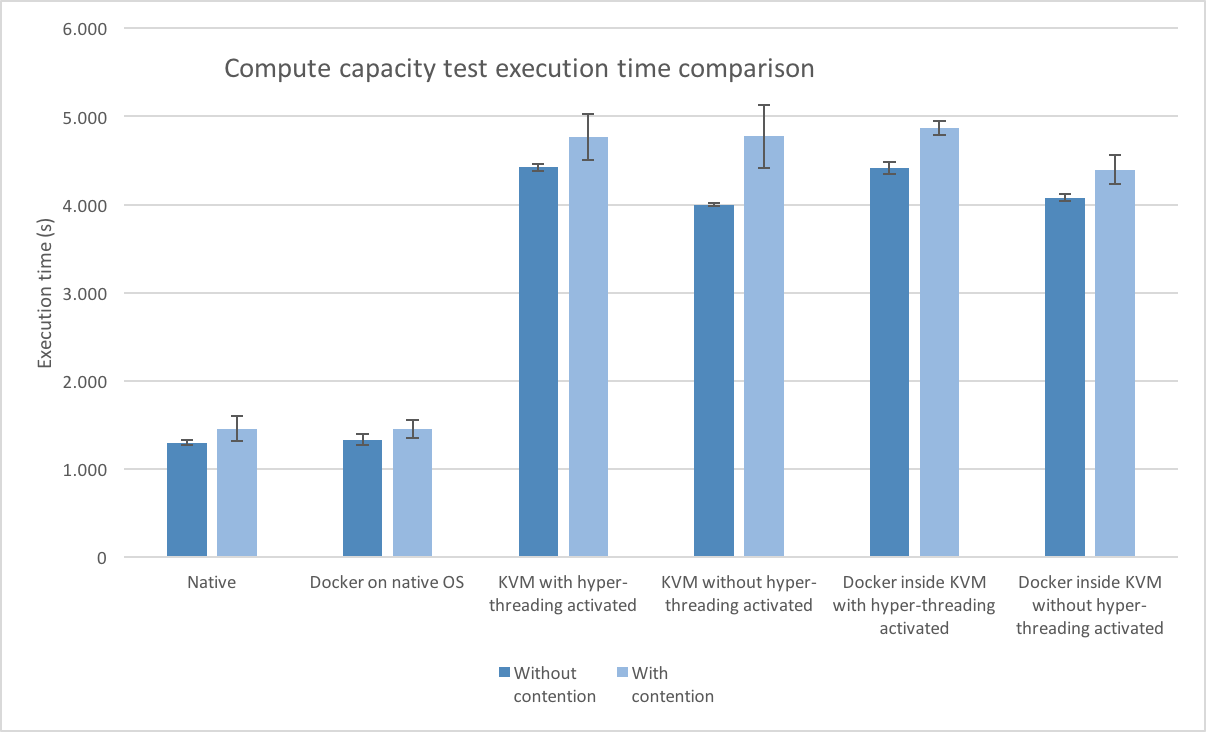
\includegraphics[width=0.75\textwidth]{chapters/measurements/images/cpu-time.png}
	\caption[Compute - resume of benchmark execution time]{Resume of benchmark execution time.}
	\label{img:measurements-cpu-results-time}
\end{figure}

As regards the execution time, we found that Docker containers are able to solve the problems
approximately in the same time as in the native execution, as Table \ref{tbl:measurements-cpu-results-time}
and chart \ref{img:measurements-cpu-results-time} shows. As we argued, this happens because
Docker containers execute at the same level of the \acs{os} on which they are based.

We have to pay specific attention to the presence or absence of Hyper-Threading Intel Technology. In fact,
keeping this feature enabled causes downgrade of the general performance.

%---------------------------------------------------------------------------------------------------
%		storage.tex
%
%	This is file contains the storage measurements.
%
%	Author: Andrea Meneghinello
% Version: 0.1
%	Table of changes:
%		21/03/2016 -> document definition
%---------------------------------------------------------------------------------------------------
\section{Storage benchmark}
\label{sec:measurements-storage}
By means of Stream benchmark tool we want to measure the \acs{ram} performance of both virtualization
environments. In order to have a basis for comparison we initially have executed the tool on the native
machine and then in various interesting environments, including:

\begin{enumerate}
	\item{one Docker container over the native \acs{os};}
	\item{one \ac{kvm} \ac{vm};}
	\item{one Docker container inside one \ac{kvm} \ac{vm}.}
\end{enumerate}

Even if running a container inside a \ac{vm} creates a double layer of virtualization, we also evaluated
this scenario because this is the only available solution if we choose a \ac{iaas} (like \ac{aws}) instead
a \ac{paas} provider.

The \acs{ram} tests were performed twice. The first time they were executed with a configuration so that
the L2-cache was exceeded. Instead, in the last one they were executed with a configuration so that the
L3-cache was exceeded.

\subsection{Stream benchmark}
\label{sec:measurements-storage-stream}
The Stream benchmark \cite{streamBenchmark} is a synthetic benchmark program that measures sustainable
memory bandwidth when performing simple operation on vectors. Performance is dominated by the memory
bandwidth of the system with the working set engineered to be significantly larger than the available
caches. The main determinants of performance are the bandwidth to main memory, and to a much lesser
extent, the cost of handling \ac{tlb} misses. The memory access pattern is regular and the hardware
pre-fetchers typically latch on to the access pattern and pre-fetch data before it is needed. Performance
is therefore gated by memory bandwidth and not by latency.

The intent of Stream is not to suggest that ``real'' applications have no data re-use, but rather to
decouple the measurement of the memory subsystem from the hypothetical ``peak'' performance of the machine.
In this respect the test is quite complementary to the Linpack benchmark test, which is typically optimized
to the point that a very large fraction of full speed is obtained on modern machines, independent of the
performance of their memory systems.

The benchmark has four components and each one adds independent information to the final results. They are:

\begin{itemize}
	\item{\keyword{\textsc{copy}}: measures transfer rates in the absence of arithmetic operations;}
	\item{\keyword{\textsc{scale}}: adds a simple arithmetic operation on the array's elements;}
	\item{\keyword{\textsc{sum}}: adds a third operand to allow multiple load/store operations;}
	\item{\keyword{\textsc{triad}}: allows chained/overlapped/fused multiply/add operations.}
\end{itemize}

Table \ref{tbl:measurements-storage-stream} gives a summary on the operations performed during the entire
execution. The different components are executed in sequence one after the other.

\begin{center}
	\begin{tabular}{| l | p{3cm} | >{\centering}m{2.5cm} | c |}
		\hline
		\textit{Name} & \textit{Operation}       & \textit{Bytes per iteration} & \textit{\acs{flops} per iteration} \\ \hline
		Copy          & $a[i] = b[i]$            & 16                           & 0                                  \\ \hline
		Scale         & $a[i] = q * b[i]$        & 16                           & 1                                  \\ \hline
		Sum           & $a[i] = b[i] + c[i]$     & 24                           & 1                                  \\ \hline
		Triad         & $a[i] = b[i] + q * c[i]$ & 24                           & 2                                  \\ \hline
	\end{tabular}
	\captionof{table}{Operation performed by Stream benchmark.}
	\label{tbl:measurements-storage-stream}
\end{center}
 
STREAM dates back to a time when floating-point arithmetic was comparable in cost to memory accesses,
so that the copy test was significantly faster than the others. This is no longer the case on any machines
of interest to \ac{hpc}, and the four Stream bandwidth values are typically quite close to each other.

\subsection{Configuration}
\label{sec:measurements-storage-configuration}
The only necessary parameter for this benchmark is the array size. To find out the correct value
in order to exceed only the L2-cache and then the L3-cache we use the following formula:

\begin{center}
	\begin{equation}
		\frac{availableCache * 1024 * 4}{8} * availableCore
	\end{equation}
\end{center}

This drives us to build an array of $16\,777\,216$ elements to exceed the L2 cache and an array of
$167\,772\,160$ elements to exceed the L3 cache.

Source code was compiled with the ``gcc'' compiler using the OpenMP directives to exploit all the
available processors.

\subsection{Results}
\label{sec:measurements-storage-results}
After executing the test in the environments described in Section \ref{sec:measurements-storage} with
the configuration described in Section \ref{sec:measurements-storage-configuration} we collected the
execution time and the sustainable memory bandwidth for each listed environments.
Tables \ref{tbl:measurements-storage-results-native}, \ref{tbl:measurements-storage-results-docker},
\ref{tbl:measurements-storage-results-kvm} and \ref{tbl:measurements-storage-results-combo} contain
the collected results about the sustainable memory bandwidth and the execution time. Charts in Figures 
\ref{img:measurements-storage-results-l2Capacity} and \ref{img:measurements-storage-results-l3Capacity}
show the available bandwidth when L2 and L3-cache are respectively exceeded by the test. Instead charts
in Figures  \ref{img:measurements-storage-results-l2Time} and \ref{img:measurements-storage-results-l3Time}
show the access time to the main memory in both test environments.

\begin{center}
	\begin{tabular}{| l | l | r | r | r | r |}
		\hline
		\multicolumn{6}{| c |}{\textbf{Native }}                                                                                                                  \\ \hline
		\multirow{2}{*}{\textit{Type}} & \multirow{2}{*}{\textit{Operation}} & \multirow{2}{*}{\textit{Rate (MB/s)}} &  \multicolumn{3}{c |}{\textit{Time (s)}}   \\ \cline{4-6}
		                               &                                     &                                       & \textit{Min} & \textit{Max} & \textit{Avg} \\ \hline
		\multirow{4}{*}{L2 overflow}   & \textit{copy}                       & $25\,290.8915$                        & $0.0106$     & $0.0145$     & $0.0128$     \\ \cline{2-6}
		                               & \textit{scale}                      & $21\,804.5532$                        & $0.0123$     & $0,0205$     & $0.0144$     \\ \cline{2-6}
		                               & \textit{add}                        & $23\,243.8253$                        & $0.0173$     & $0.0225$     & $0.0191$     \\ \cline{2-6}
		                               & \textit{triad}                      & $23\,930.1989$                        & $0.0168$     & $0.0213$     & $0.0185$     \\ \hline
		\multirow{4}{*}{L3 overflow}   & \textit{copy}                       & $34\,888.0418$                        & $0.0769$     & $0.0807$     & $0.0779$     \\ \cline{2-6}
		                               & \textit{scale}                      & $35\,002.6863$                        & $0.0783$     & $0.0816$     & $0.0783$     \\ \cline{2-6}
		                               & \textit{add}                        & $39\,904.2086$                        & $0.1009$     & $0.1031$     & $0.1013$     \\ \cline{2-6}
		                               & \textit{triad}                      & $39\,946.1155$                        & $0.1008$     & $0.1031$     & $0.1026$     \\ \hline
	\end{tabular}
	\captionof{table}{Resume of benchmark on native}
	\label{tbl:measurements-storage-results-native}
\end{center}

\begin{center}
	\begin{tabular}{| l | l | r | r | r | r |}
		\hline
		\multicolumn{6}{| c |}{\textbf{Docker }}                                                                                                                  \\ \hline
		\multirow{2}{*}{\textit{Type}} & \multirow{2}{*}{\textit{Operation}} & \multirow{2}{*}{\textit{Rate (MB/s)}} &  \multicolumn{3}{c |}{\textit{Time (s)}}   \\ \cline{4-6}
		                               &                                     &                                       & \textit{Min} & \textit{Max} & \textit{Avg} \\ \hline
		\multirow{4}{*}{L2 overflow}   & \textit{copy}                       & $17\,957.7955$                        & $0.0149$     & $0.0196$     & $0.0176$     \\ \cline{2-6}
		                               & \textit{scale}                      & $18\,157.0402$                        & $0.0148$     & $0.0219$     & $0.0183$     \\ \cline{2-6}
		                               & \textit{add}                        & $18\,965.3995$                        & $0.0212$     & $0.0271$     & $0.0239$     \\ \cline{2-6}
		                               & \textit{triad}                      & $19\,480.1359$                        & $0.0207$     & $0.0284$     & $0.0241$     \\ \hline
		\multirow{4}{*}{L3 overflow}   & \textit{copy}                       & $34\,942.0707$                        & $0.0768$     & $0.0870$     & $0.0807$     \\ \cline{2-6}
		                               & \textit{scale}                      & $34\,577.0054$                        & $0.0776$     & $0.0949$     & $0.0847$     \\ \cline{2-6}
		                               & \textit{add}                        & $39\,856.8392$                        & $0.1010$     & $0.1227$     & $0.1084$     \\ \cline{2-6}
		                               & \textit{triad}                      & $39\,917.6961$                        & $0.1009$     & $0.1183$     & $0.1183$     \\ \hline
	\end{tabular}
	\captionof{table}{Resume of benchmark on Docker container}
	\label{tbl:measurements-storage-results-docker}
\end{center}

\begin{center}
	\begin{tabular}{| l | l | r | r | r | r |}
		\hline
		\multicolumn{6}{| c |}{\textbf{\ac{kvm} \ac{vm} }}                                                                                                        \\ \hline
		\multirow{2}{*}{\textit{Type}} & \multirow{2}{*}{\textit{Operation}} & \multirow{2}{*}{\textit{Rate (MB/s)}} &  \multicolumn{3}{c |}{\textit{Time (s)}}   \\ \cline{4-6}
		                               &                                     &                                       & \textit{Min} & \textit{Max} & \textit{Avg} \\ \hline
		\multirow{4}{*}{L2 overflow}   & \textit{copy}                       & $16\,728.0764$                        & $0.0160$     & $0.0232$     & $0.0203$     \\ \cline{2-6}
		                               & \textit{scale}                      & $14\,775.9771$                        & $0.0182$     & $0.0238$     & $0.0199$     \\ \cline{2-6}
		                               & \textit{add}                        & $15\,341.6046$                        & $0.0262$     & $0.0311$     & $0.0282$     \\ \cline{2-6}
		                               & \textit{triad}                      & $18\,268.3036$                        & $0.0220$     & $0.0310$     & $0.0270$     \\ \hline
		\multirow{4}{*}{L3 overflow}   & \textit{copy}                       & $34\,942.0707$                        & $0.1325$     & $0.1768$     & $0.1549$     \\ \cline{2-6}
		                               & \textit{scale}                      & $34\,577.0054$                        & $0.1390$     & $0.1606$     & $0.1518$     \\ \cline{2-6}
		                               & \textit{add}                        & $39\,856.8392$                        & $0.1827$     & $0.2428$     & $0.2011$     \\ \cline{2-6}
		                               & \textit{triad}                      & $39\,917.6961$                        & $0.1751$     & $0.2066$     & $0.1965$     \\ \hline
	\end{tabular}
	\captionof{table}{Resume of benchmark on \acs{kvm} \acs{vm}}
	\label{tbl:measurements-storage-results-kvm}
\end{center}

\begin{center}
	\begin{tabular}{| l | l | r | r | r | r |}
		\hline
		\multicolumn{6}{| c |}{\textbf{Docker container inside a \ac{kvm} \ac{vm}}}                                                                               \\ \hline
		\multirow{2}{*}{\textit{Type}} & \multirow{2}{*}{\textit{Operation}} & \multirow{2}{*}{\textit{Rate (MB/s)}} &  \multicolumn{3}{c |}{\textit{Time (s)}}   \\ \cline{4-6}
		                               &                                     &                                       & \textit{Min} & \textit{Max} & \textit{Avg} \\ \hline
		\multirow{4}{*}{L2 overflow}   & \textit{copy}                       & $17\,025.0394$                        & $0.0158$     & $0.0283$     & $0.0192$     \\ \cline{2-6}
		                               & \textit{scale}                      & $16\,022.2554$                        & $0.0168$     & $0.0314$     & $0.0205$     \\ \cline{2-6}
		                               & \textit{add}                        & $21\,185.5672$                        & $0.0190$     & $0.0369$     & $0.0251$     \\ \cline{2-6}
		                               & \textit{triad}                      & $20\,452.8098$                        & $0.0197$     & $0.0391$     & $0.0243$     \\ \hline
		\multirow{4}{*}{L3 overflow}   & \textit{copy}                       & $17\,133.2818$                        & $0.1567$     & $0.1975$     & $0.1701$     \\ \cline{2-6}
		                               & \textit{scale}                      & $20\,331.0000$                        & $0.1320$     & $0.2177$     & $0.1641$     \\ \cline{2-6}
		                               & \textit{add}                        & $23\,684.9061$                        & $0.1700$     & $0.2359$     & $0.2074$     \\ \cline{2-6}
		                               & \textit{triad}                      & $20\,177.8757$                        & $0.1996$     & $0.2393$     & $0.2197$     \\ \hline
	\end{tabular}
	\captionof{table}{Resume of benchmark on a container inside a \acs{kvm} \acs{vm}}
	\label{tbl:measurements-storage-results-combo}
\end{center}

From charts \ref{img:measurements-storage-results-l3Capacity} and \ref{img:measurements-storage-results-l3Time}
we can assert that the \acs{os}-level virtualization provided by Docker containers is able to access
to the main memory almost in the same time of the native execution and it is able to exploit completely
the available bandwidth. Instead the hardware-level virtualization, provided by \ac{kvm} splits in half
the bandwidth and doubles the access time to the main memory. This is due to the overhead introduced by
hypervisor.

\begin{figure}
	\centering{}
	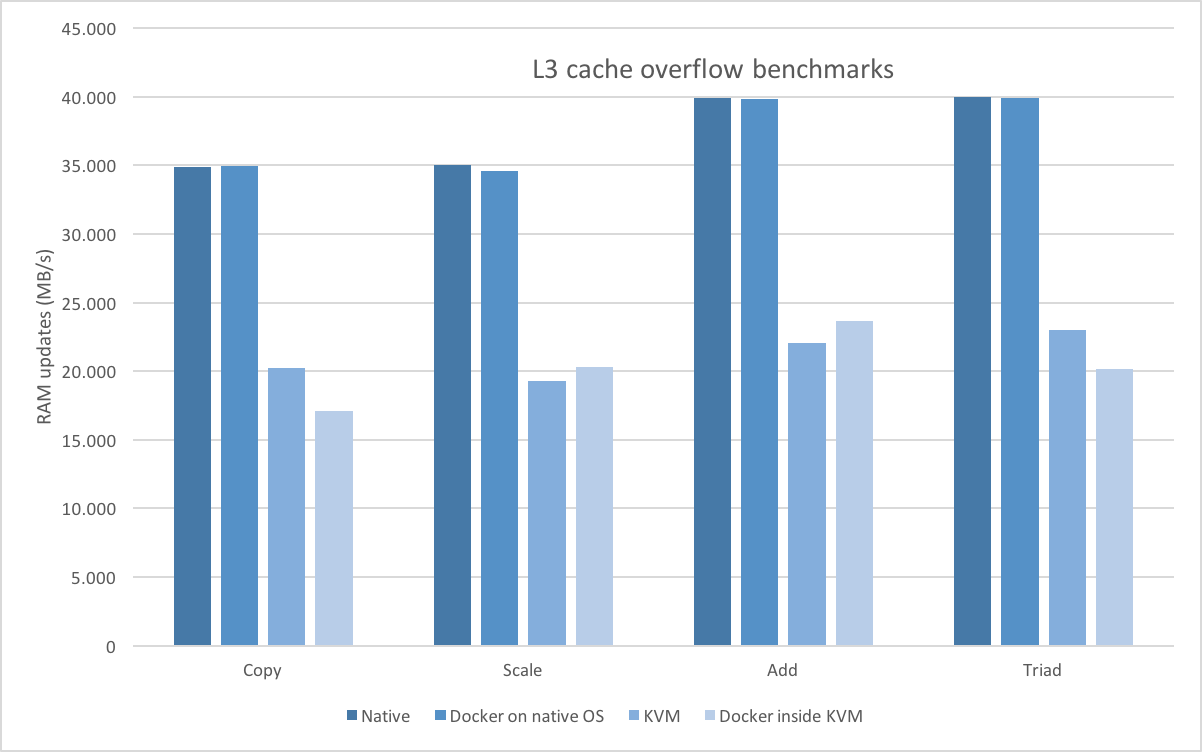
\includegraphics[width=0.8\textwidth]{chapters/measurements/images/storage-l3-capacity.png}
	\caption[Storage - overflow L3 cache]{Resume of benchmark when the L3 cache is exceeded}
	\label{img:measurements-storage-results-l3Capacity}
\end{figure}

Also in this case executing a Docker container inside a \ac{kvm} \ac{vm} do not produce a substantial
downgrade of the performance with respect to the execution without Docker in the \ac{vm}. Also in this
scenario we have demonstrated that the \acs{os}-level virtualization layer is not officious.

\begin{figure}
	\centering{}
	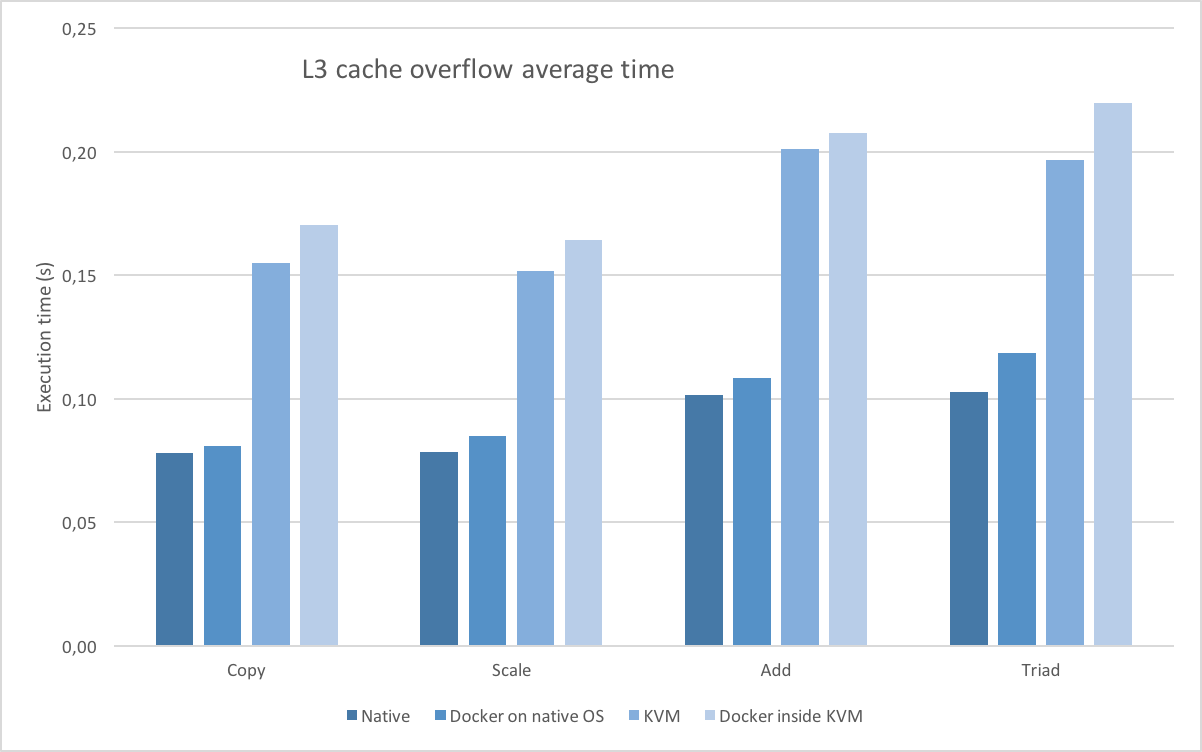
\includegraphics[width=0.8\textwidth]{chapters/measurements/images/storage-l3-time.png}
	\caption[Storage - access time L2 cache exceeded]{Resume of memory access time when the L2
		cache is exceeded.}
	\label{img:measurements-storage-results-l3Time}
\end{figure}

Instead, analysing charts illustrated in Figure \ref{img:measurements-storage-results-l2Capacity}
and \ref{img:measurements-storage-results-l2Time} when only L2 cache is exceeded the performance are
downgraded almost in the same way in all the tested scenarios regard to native execution. This is
imputable to the position of data in the caches associated to each core.

\begin{figure}
	\centering{}
	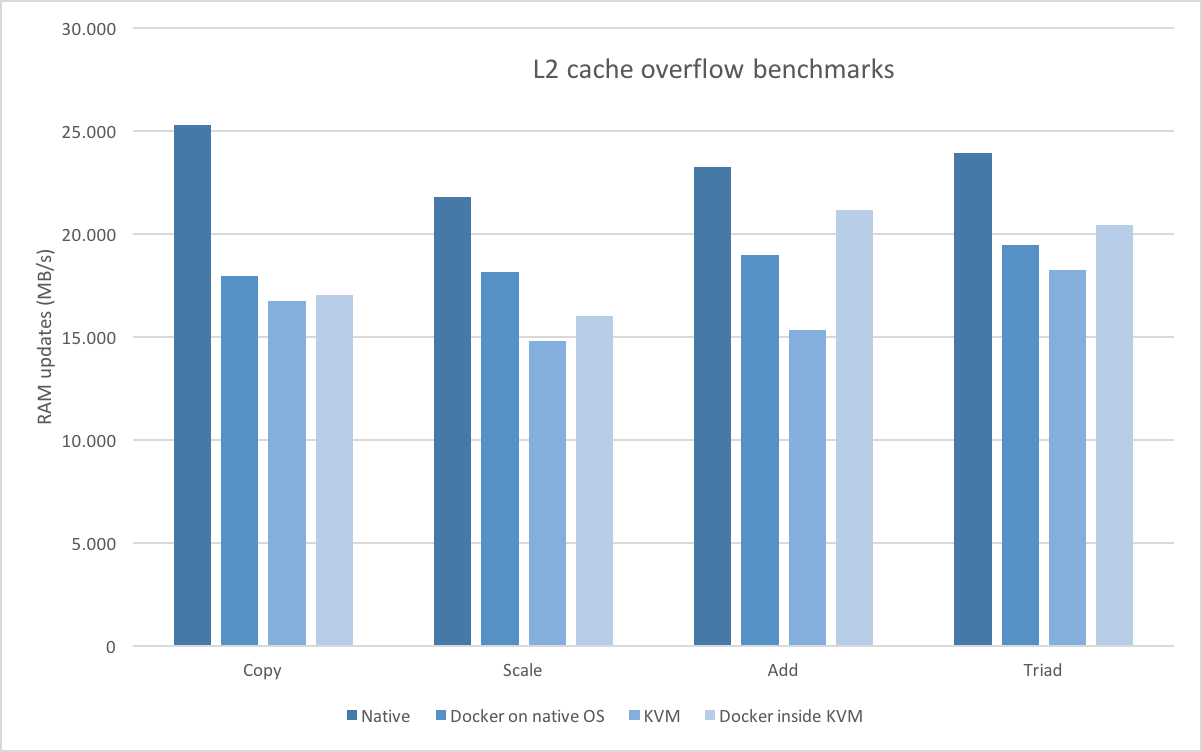
\includegraphics[width=0.8\textwidth]{chapters/measurements/images/storage-l2-capacity.png}
	\caption[Storage - overflow L2 cache]{Resume of benchmark when the L2 cache is exceeded}
	\label{img:measurements-storage-results-l2Capacity}
\end{figure}

\begin{figure}
	\centering{}
	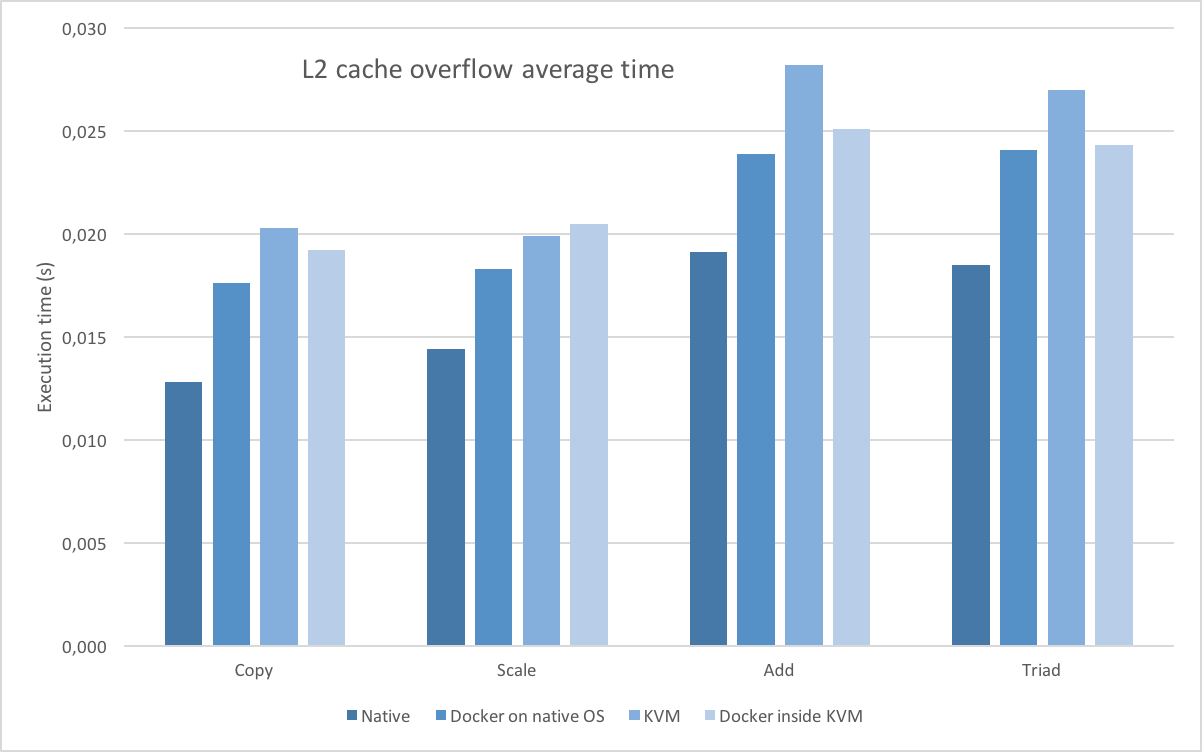
\includegraphics[width=0.8\textwidth]{chapters/measurements/images/storage-l2-time.png}
	\caption[Storage - access time L2 cache exceeded]{Resume of memory access time when the L2
		cache is exceeded.}
	\label{img:measurements-storage-results-l2Time}
\end{figure}

%---------------------------------------------------------------------------------------------------
%		network.tex
%
%	This is file contains the network measurements.
%
%	Author: Andrea Meneghinello
% Version: 0.1
%	Table of changes:
%		21/03/2016 -> document definition
%---------------------------------------------------------------------------------------------------
\section{Network benchmark}
\label{sec:measurements-network}
By means of Iperf benchmark tool we want to measure how the different virtualization environments
can exploit the available bandwidth and the network latency. In order to have a basis for comparison 
we initially have executed the tests on the two native machines and then in the following environments:

\begin{enumerate}
	\item{two Docker containers placed in different physical machines;}
	\item{two \ac{kvm} \ac{vm}s placed in different physical machines.}
\end{enumerate}

As previously said in the chapter introduction, the two physical machines are linked together in a \acs{lan}
through a Netgear M7300 series Gigabit switch by means of optical fibre cables.

\subsection{Iperf benchmark}
\label{sec:measurements-network-nuttcp}
Iperf \cite{iperfBenchmark} is a network performance measurement tool intended for use by network and
system managers. Its most basic usage is to determine the raw \acs{tcp} (or \acs{udp}) network layer
throughput by transferring memory buffers from a source system across an interconnecting network to a
destination system, either transferring data for a specified time interval, or alternatively transferring
a specified number of bytes. In addition to reporting the achieved network throughput in Mbps, iperf also
provides additional useful information related to the data transfer such as user, system, and wall-clock time,
transmitter and receiver \acs{cpu} utilization, and loss percentage (for \acs{udp} transfers).

Iperf allows network managers to set various parameters that can be used for testing, optimizing
or tuning a network. Iperf has a \keyword{client} and \keyword{server} functionality, and can
measure the throughput between the two ends, either unidirectionally or bi-directionally. Typical Iperf output
contains a time-stamped report of the amount of data transferred and the throughput measured.

\subsection{Configuration}
\label{sec:measurements-network-configuration}
To measure both the network bandwidth and latency we have used similar network configurations. When we have
tested the network bandwidth, we do not have forced the tool with any parameter, so it was able to adjust network
parameters, like network windows, automatically.

Instead, when we had measured the network latency we have configured the tool so that it was able to send
a packet and wait for the server response before it could send another request. Thus only one transaction is
in flight at a time. 

\subsection{Results}
\label{sec:measurements-network-result}
After executing the tests in all the environments we collected the results that are shown in Table
\ref{tbl:measurements-network-result-bandwidth} in the matter of the available network bandwidth, and
in Table \ref{tbl:measurements-network-result-latency} for those about the network latency.

\begin{center}
	\begin{tabular}{| l | c | r | r | r | r |}
		\hline
		\multicolumn{6}{| c |}{\textbf{Network throughput}}                                                                  \\ \hline
		\multicolumn{2}{| c |}{}                        &          \multicolumn{4}{c |}{\textit{Throughput (MB/s)}}          \\ \hline
		\textit{Env.}              & \textit{Direction} & \textit{Min}  & \textit{Max}  & \textit{Avg}  & \textit{Std. Dev.} \\ \hline
		\multirow{2}{*}{Native}    & C -> S             & $9\,409.8646$ & $9\,415.2581$ & $9\,414.6153$ & $0.6711$           \\ \cline{2-6}
		                           & S -> C             & $9\,410.3983$ & $9\,415.2769$ & $9\,414.6119$ & $0.6065$           \\ \hline
		\multirow{2}{*}{Docker}    & C -> S             & $9\,391.9720$ & $9\,394.8341$ & $9\,393.4361$ & $0.8175$           \\ \cline{2-6}
		                           & S -> C             & $9\,389.4003$ & $9\,391.3858$ & $9\,390.3264$ & $0.5636$           \\ \hline
		\multirow{2}{*}{\acs{kvm}} & C -> S             & $9\,356.8689$ & $9\,358.8478$ & $9\,357.8673$ & $0.5469$           \\ \cline{2-6}
		                           & S -> C             & $9\,353.4524$ & $9\,355.3841$ & $9\,354.4433$ & $0.5720$           \\ \hline
	\end{tabular}
	\captionof{table}{Network available bandwidth.}
	\label{tbl:measurements-network-result-bandwidth}
\end{center}

From the chart, illustrated in Figure \ref{img:measurements-network-results-bandwidth}, we can observe
that in matter of network bandwidth there are not substantial differences, given that all the
virtualization environments are able to get close to the theoretical limit of 9.4 Gb/s\footnote{Limit
forced by the configuration of the \acs{tcp} network protocol.}. The pattern is maintained in both
directions (client to server one and viceversa). This leads us to affirm that the virtualization
layer does not compromise the available bandwidth in both the virtualization environments.

\begin{figure}
	\centering{}
	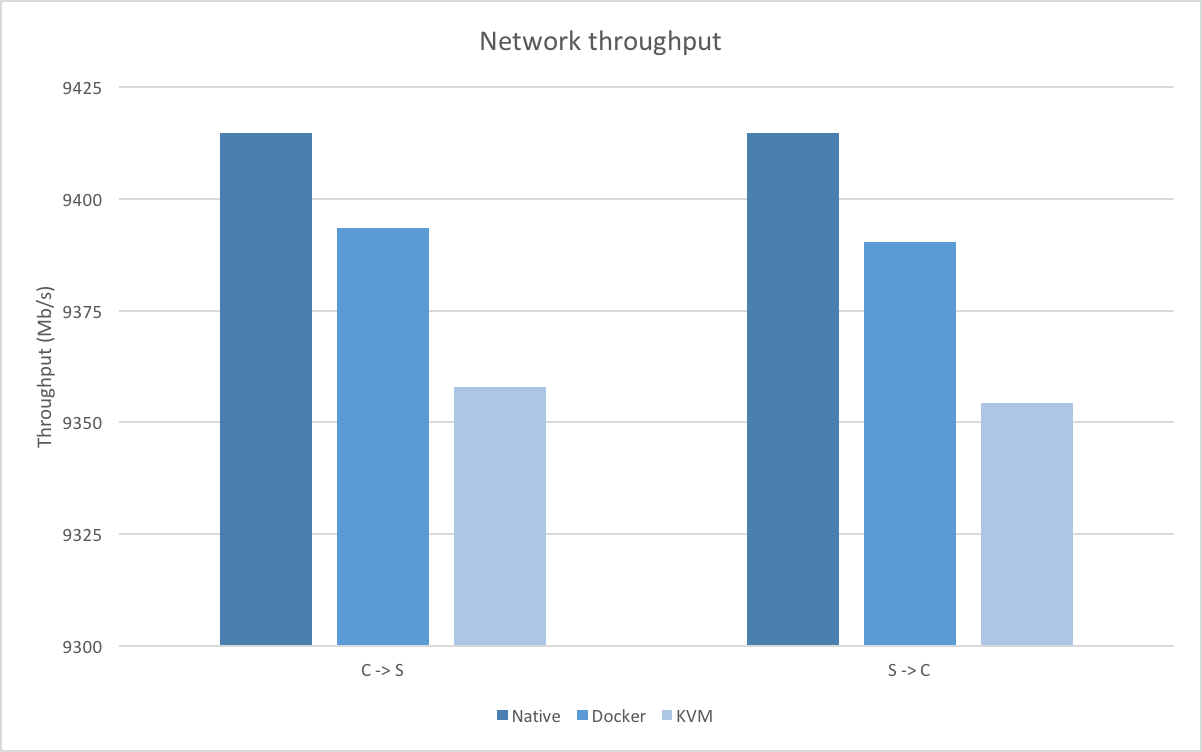
\includegraphics[width=0.7\textwidth]{chapters/measurements/images/network-throughput.png}
	\caption[Network - avaialable bandwidth]{Network available bandwidth measured.}
	\label{img:measurements-network-results-bandwidth}
\end{figure}

With respect to the network delay we have found that the \acs{os}-level virtualization, provided by 
Docker, is the one that creates the greatest delay (as Figure
\ref{img:measurements-network-results-latency} shows); it is higher, even if just a little, than the one
provided by the hardware-level virtualization which is twice that of native execution.

\begin{center}
	\begin{tabular}{| l | r | r | r | r |}
		\hline
		\multicolumn{5}{| c |}{\textbf{Network Latency}}                                \\ \hline
		&         \multicolumn{4}{c |}{\textit{Latency ($\mu$s)}}         \\ \hline
		\textit{Env.} & \textit{Min} & \textit{Max} & \textit{Avg} & \textit{Std. Dev.} \\ \hline
		Native        & $37.2296$    & $41.9557$    & $39.4489$    & $1.5114$           \\ \hline
		Docker        & $73.0843$    & $79.8891$    & $76.2959$    & $1.8605$           \\ \hline
		\acs{kvm}     & $69.0498$    & $74.9104$    & $71.8517$    & $1.4772$           \\ \hline
	\end{tabular}
	\captionof{table}{Network latency resume.}
	\label{tbl:measurements-network-result-latency}
\end{center}

\begin{figure}
	\centering{}
	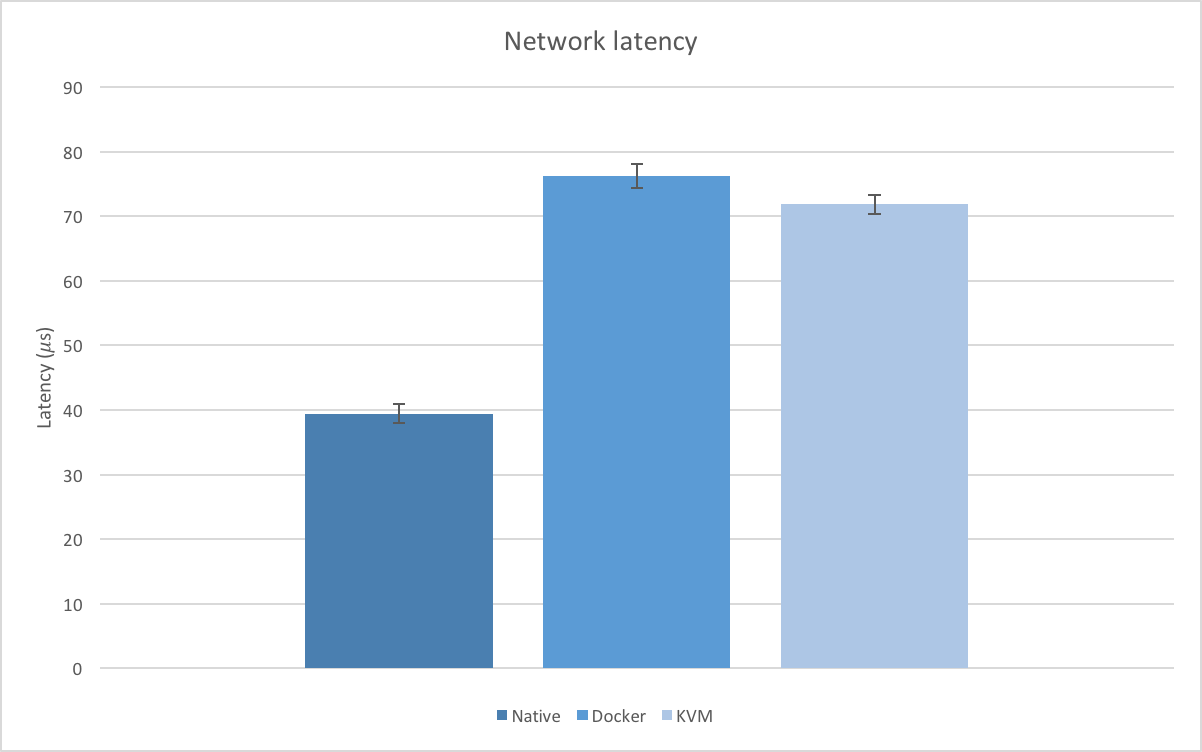
\includegraphics[width=0.7\textwidth]{chapters/measurements/images/network-latency.png}
	\caption[Network - latency measured]{Network latency measured.}
	\label{img:measurements-network-results-latency}
\end{figure}

To investigate the causes that generate this lack in performance we have analysed the stacks that divide
both the \acs{os}-level virtualization and the hardware-level virtualization from the physical world (the
different stacks are illustrated in Figure \ref{img:measurements-network-result-stacks}). Reading also
the official Docker documentation we have found that during the Docker daemon installation, on the system,
a network bridge (named ``Docker$0$'') is created. Later this bridge is linked to one of the available
\ac{nic} card of the system so that the container is able to send and receive data over the network (In
our test cases it was hooked to ``p1p2'' interface linked to the network switch).

This configuration creates a double layer of translation because both the Docker daemon and the \ac{nic}
use the \ac{nat} service. In particular, both the bridge (``Docker$0$'') and the \ac{nic} have a
private \acs{ip} address that must be translated before a container can send data over the real network.
The first translation binds a \acs{tcp} port of the container with the bridge address, while the second
one binds the private \acs{ip} address of the bridge with the private \acs{ip} address of the \ac{nic}.

The Docker ecosystem is default configured to use the \ac{nat} technique to communicate with the outside
world and this is the origin cause of the measured delay. This default behaviour is changeable\footnote{
Remember the Docker school of though ``battery included, but swappable''.} in order to ``attach''
containers directly over the \ac{nic}, but this solution introduces security issues that must be
considered. In the following chapter we will see a possible network architecture that considers these
aspects but lowering at the same time the network delay.

\begin{figure}
	\centering{}
	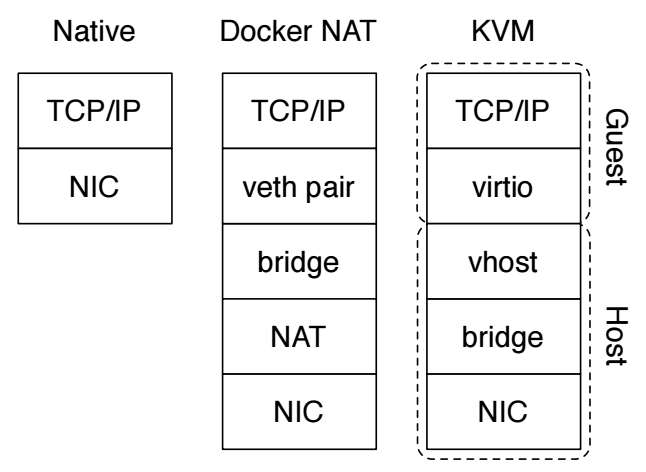
\includegraphics[width=0.5\textwidth]{chapters/measurements/images/network-stack.png}
	\caption[Network stack in different environments]{Network stack in different virtualization
		environments.}
	\label{img:measurements-network-result-stacks}
\end{figure}

%---------------------------------------------------------------------------------------------------
%		summary.tex
%
%	This is file contains the chapter summary.
%
%	Author: Andrea Meneghinello
% Version: 0.1
%	Table of changes:
%		21/03/2016 -> document definition
%---------------------------------------------------------------------------------------------------
\section{Summary}
\label{sec:measurements-summary}
After the execution of the tests and have analysed the collected results we can now derive some conclusion
about the two virtualization technologies: \ac{kvm} \ac{vm}s and Docker containers. 

Both are, nowadays, mature technologies that have benefited of incremental hardware and software updates.
In general, we can assert that there is, at most, a point of view that is advantageous for the hardware-virtualization
level technologies and others that are more appropriate for the \acs{os}-virtualization level ones.

If we look at the hardware performance we can observe that the Docker containers are able to exploit very well
the available underlying hardware, except for the network delay (see Section \ref{sec:measurements-network-result}).
Instead, in matter of adapt themselves to share the underlying available resources, we found that the
\ac{vm}s are more mature than the counterpart.

After working a little bit with Docker technology, we have appreciated its lightweight, the rapidity that
it follows, and the easy \acs{api} that they provide to developers. Even though the Docker container are more
recent than the \ac{kvm} \ac{vm}s, they provide to developers a good level of virtualization and make some tasks
more easier (like build environments.) We expect that in nearly future this technology will be improved and largely
preferred by many developers. 

As we asserted in the previous chapter, the only adoption of a good virtualization layer, that is able to exploit
the underlying hardware, is not sufficient to guarantee good levels of elasticity. Because of this, in the next
chapter, aware of the experience matured with the performed tests, we want to introduce a possible software
architecture that can provide good level of elasticity combined with the \acs{os}-virtualization level and that
lead developers to easily generate multi-tenants applications. 